\subsection{Acetaldeide - CAS 10 elettroni / 7 orbitali}

Al fine di migliorare la trattazione sull'acetaldeide, si \`e quindi scelto
uno spazio attivo compatibile con la necessit\`a di includere il doppietto $n_y$
sia nello stato fondamentale che nello stato eccitato.

La scelta ha portato ad ampliare lo spazio attivo, fino ad avere
5 orbitali A$^{\prime}$ e 2 orbitali A$^{\prime\prime}$,
e uno spazio di core costituito da 6 orbitali di simmetria A$^{\prime}$
e 1 orbitale di simmetria A$^{\prime\prime}$.
Con questa definizione, sono necessarie 106 configurazioni
nell'espansione CAS-CI, contro le 28 del precedente spazio attivo.

I risultati ottenuti sono rappresentati in tabella \ref{tab:acetaldeide_vertical_basis_7}
\begin{center}
\begin{threeparttable}
\caption{\small Acetaldeide - Energia di transizione verticale $n_y \rightarrow \pistar$ di singoletto, CAS 10 elettroni 7 orbitali}
\label{tab:acetaldeide_vertical_basis_7}
\small
\begin{tabular}{|c|ccc|ccc|}
\hline
Basis	& \multicolumn{3}{c|}{GS\tnote{1}}				& \multicolumn{3}{c|}{$n_y \rightarrow \pistar$ vert.\tnote{2}} \\
		& CASSCF		& NEV-PT	 	&	NEV-PT		& CASSCF		& NEV-PT	& NEV-PT	  \\
		& 				& SC 			&	PC			& 				& SC		& PC	 	 \\
\hline
6-31G	& 0.927916		& 1.138181		&	1.140489	& 4.06			& 4.01		& 4.03		\\
cc-pVDZ	& 1.004396		& 1.370583		&	1.373364	& 4.58			& 4.37		& 4.38		\\
ano-1	& 1.042885		& 1.405010		&	1.408962	& 4.59			& 4.35 		& 4.34		\\
6-311G*	& 1.026837		& 1.445053		&	1.447570	& 4.62			& 4.35		& 4.37		\\
cc-pVTZ & 1.050199		& 1.556482		&	1.559922	& 4.62			& 4.32		& 4.32		\\			
\hline
\hline
Exp.\tnote{3}&				& 				& 				& \multicolumn{3}{c|}{4.28} \\
\hline
\end{tabular}
\begin{tablenotes}
 \item[1] Energia come -(152 + valore) Hartree
 \item[2] Valori in eV
 \item[3] Cfr. \cite{jpc-97-17-1993-4293}
\end{tablenotes}
\end{threeparttable}
\end{center}

\`E evidente come, con uno spazio attivo allargato, si venga incontro alla
necessit\`a fisica di descrivere lo stato fondamentale e quello eccitato
nello stesso modo. I valori per la transizione a livello CAS restano
tuttavia relativamente distanti dal valore vero di 4.28 eV, nonostante il
numero di configurazioni sia considerevolmente aumentato. La perturbazione
consente di recuperare parte dell'energia di correlazione ed avvicinarsi
cos\`i in modo pi\`u deciso all'energia di transizione sperimentale.

Analoghe considerazioni per quanto riguarda la transizione adiabatica,
i cui risultati sono riportati in tabella \ref{tab:acetaldeide_adiab_basis_7}

\begin{center}
\begin{threeparttable}
\caption{\small Acetaldeide - Energia di transizione adiabatica $n_y \rightarrow \pistar$ di singoletto, CAS 10 elettroni 7 orbitali}
\label{tab:acetaldeide_adiab_basis_7}
\small
\begin{tabular}{|c|ccc|ccc|}
\hline
Basis	& ZPE 			& ZPE 			& $\Delta$ZPE		& CASSCF		& NEV-PT		& NEV-PT	 \\
		& (GS)			& (Ecc.) 		& 					& ZPE			& SC/ZPE		& PC/ZPE 	 \\
\hline
6-31G	& 1.612			& 1.544			& -0.068			& 3.32			& 3.30			& 3.33			 \\
cc-pVDZ & 1.592			& 1.531			& -0.062			& 3.73 			& 3.64			& 3.66			 \\
ano-1	& 1.603			& 1.542			& -0.060			& 3.73			& 3.60 			& 3.61			 \\
6-311G* & 1.600 		& 1.543			& -0.057			& 3.74			& 3.65			& 3.66			 \\
cc-pVTZ & 1.590			& 1.531			& -0.059			& 3.76			& 3.68			& 3.69			 \\
\hline
\hline
Exp.\tnote{1}&				& 				& 					& \multicolumn{3}{c|}{3.69} \\
\hline
\end{tabular}
\begin{tablenotes}
 \item[1] Cfr. \cite{jpc-97-17-1993-4293}
 \item[] Valori in eV
\end{tablenotes}
\end{threeparttable}
\end{center}

Come si pu\`o vedere, c'\`e un ottimo accordo tra il dato sperimentale e il
valore calcolato, gi\`a buono a livello CAS, che viene migliorato ulteriormente
dall'applicazione della perturbazione.

Al solito, i grafici \ref{fig:acetaldeide_energie_vert_7} e \ref{fig:acetaldeide_energie_adiab_7}
mostrano l'andamento dei dati sopra rappresentati, permettendo di
evidenziare in modo pi\`u netto l'andamento delle energie di transizione
verticale e adiabatica
\begin{figure}[ht]
\begin{center}
\includegraphics[angle=270,width=11cm,keepaspectratio]{immagini/acetaldeide/energie_vert_7.eps}
\parbox[h]{12cm}{
\caption{\small Acetaldeide - energia di transizione verticale su basi differenti a livello CASSCF (linea rossa), NEV-PT/SC (linea verde) e NEV-PT/PC (linea blu) come funzione della base atomica.}
\label{fig:acetaldeide_energie_vert_7}
}
\end{center}
\end{figure}
\pagebreak
\begin{figure}[ht]
\begin{center}
\includegraphics[angle=270,width=12cm,keepaspectratio]{immagini/acetaldeide/energie_adiab_7.eps}
\parbox[h]{12cm}{
\caption{\small Acetaldeide - energia di transizione adiabatica su basi differenti a livello CASSCF (linea rossa), NEV-PT/SC (linea verde) e NEV-PT/PC (linea blu) come funzione della base atomica.}
\label{fig:acetaldeide_energie_adiab_7}
}
\end{center}
\end{figure}

\clearpage
